% !TeX root = ../main.tex

\chapter{绪论}

\section{研究背景与研究意义}
移动智能机器人是人工智能大背景下的热门研究方向,也是未来国际化竞争的重要方向,随着科技的飞速发展,智能化技术将开启下一个工业革命的大门。谁能在无人智能化技术上领先,谁便在未来的国际话语竞争与产业升级中掌握先机。“中国制造2025计划”将高新技术产业作为国家战略之一,而移动智能机器人技术作为高新技术的核心体现之一,自有其璀璨之处。移动智能机器人技术是一门集硬件科学、定位与导航技术、测量与建图科学等相关学科为一体的交叉技术,是一个由传感器、执行器、电源管理以及软件算法组成的复杂控制系统,同时,具备环境感知、路径规划、动态分析、移动避障等多种功能于一体。广义上的移动智能机器人技术包含了无人驾驶、无人配送等多个应用技术方向,除了这些简单的生活用途之外,医疗机器人、战争无人车等特殊用途的机器人也逐渐登上舞台。目前在移动智能机器人技术的应用方向上,走在前沿的技术公司已经有了相当惊艳的产品。一些明星公司例如百度、智行者、酷哇机器人、波士顿等的代表产品如图1.1所示。

\begin{figure}[ht]
  \centering
  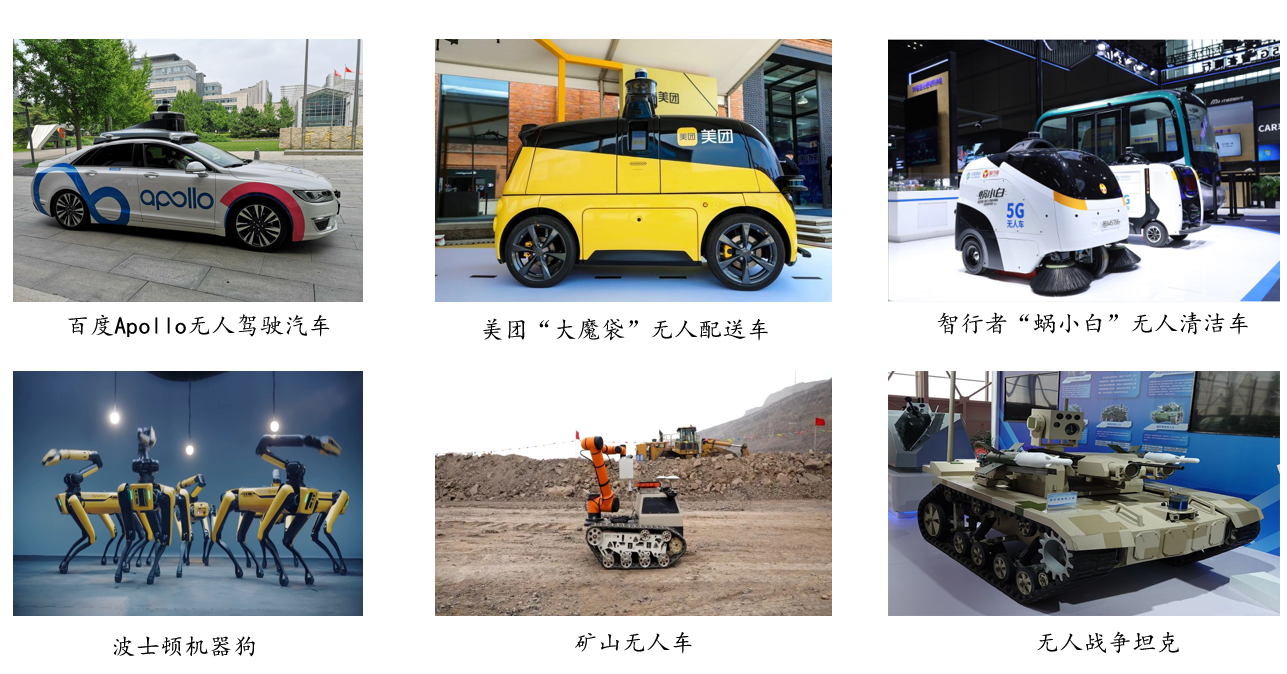
\includegraphics[scale=0.5]{cars.jpg}
  \caption{用于各种场景的移动智能机器人}
\end{figure}

在移动智能机器人领域,移动机器人得到了最广泛的关注与研究。移动机器人的导航技术是其实现目的性运动的最基础功能之一,依托于环境感知、路径规划、定位建图等多个模块的复杂信息,整合信息后将控 制信号下发给执行器件,最终完成移动移动机器人的有目的性运动。可以认为导航系统是移动机器人由单纯的实验室验证模型走向功能性使用的第一步也是最关键的一步。随着劳动力市场的用人成本大幅度提升,使用移动机器人代替工人进行重复、无聊的工作成了提高生产效率,节约生产成本的重要途径。例如,目前移动机器人在多个园区已经开展了无人配送、无人清扫等多方面的广泛应用,而在这个过程中,移动机器人的导航技术则是这些功能实现的前提,导航技术的最根本任务就是依托指令的目的化运行,导航技术将移动智能机器人从以往的点对点单一指令化工作,提升至目前可在封闭园区内(甚至开放场景下)动态地避开行人等动态障碍物,实施规划、随机应变地完成非固定化路线的导航任务。在移动机器人的最基础功能中,导航系统因其本身在无人设备或系统上的泛化应用,得到了多方机构乃至高校实验室的研究青睐。不仅是在生产过程中,在救火救灾、抢险以及特种任务中,智能无人平台都发挥了巨大的优势。2020年初的突发疫情,更是为移动智能机器人的发展提供了舞台。在国内外多处人流密集场所,封控小区以及其他对非必要性人为接触有需求的场合,智能无人平台凭借其出色的运动性能,获得了多家医院以及酒店的使用青睐。我们有理由相信,在我们国家取得了伟大的疫情防控胜利的成果之中,移动智能机器人的贡献是极大的。目前的移动机器人已经应用在了各行各业之中,伴随着移动机器人的应用,导航系统的发展也与时俱进。以往的导航系统仅仅是简单的对目的地的响应,而随着移动机器人的应用环境愈发复杂:从室内到室外,从静态环境到动态环境,从小范围使用到园区场景下部署,每一次场景的改变,都对移动机器人的导航系统产生了极大的要求,也对导航系统的性能提出了更为严苛的挑战。

为了响应国家“中国制造2025计划”的号召,同时因我的研究生生涯都在疫情中度过,深刻认识到了移动机器人技术在园区场景下的广泛应用的意义,本文旨在围绕校园场景下这一园区环境的代表性场所,研究并且设计开发出一套适合本地校园场景等园区场景下的导航系统,满足师生日常对于配送、定点货运以及危险科研任务等实地需求。在此过程中,解决局部最优以及园区场景下动态物体较多等重大问题,是本研究的亮点,同时也是探索移动机器人技术在园区场景下的延申需求关键突破。


\section{移动机器人导航系统研究现状及其分析}
移动机器人的导航系统是指移动机器人在接收到目的地信息后,对目标点信息处理,根据自身实时定位,在可行驶区域上规划从当前位置到达目标点位置的可行使路径,并且沿着既定路径行驶,期间通过激光雷达或者视觉信息实时感知周边环境,对外部环境的改变做出实时反应,安全高效、无碰撞地到达目标点的功能系统。移动机器人的导航系统是无人车类智能化系统的最基础、最关键技术。一般来说,任何无人智能设备的导航系统需要结合多个底层模块的功能,加工处理多种输入输出信息,而后将已有信息作为输入,通过导航系统的计算,输出相应的系统控制信息给到执行部件,最终完成智能无人设备的导航功能。由于导航系统上连无人设备的信息决策层,下至底盘、激光雷达等硬件层,所以导航系统是一个复杂的耦合系统。本部分会对导航系统的需求进行进行分析,并阐述导航系统的发展历程,关注在移动机器人导航系统在各个发展阶段的代表性作品,分析各阶段方法的优缺点。最后,对现有导航系统的问题进行总结归纳,并对导航系统最关键的安全性问题上进行着重分析,并给出解决方案。

\subsection{移动机器人导航系统的发展历程}
移动机器人的导航技术是一项综合性交叉技术,主要分为前端感知、建图定位、路径规划、以及决策执行等模块。最早的移动机器人出现于20世纪中叶,此时距离汽车的发明已经过去了半个多世纪,随着早期汽车的成熟,智能化汽车的概念应运而生。1956年,美国通用汽车公司制造出了第一辆无人车实体Firebird II,并首次提出自动导航的概念。在第一辆移动机器人问世后第十年,美国斯坦福大学的研究所SRI人工智能研究中心研发出具有车轮结构的机器人Shakey,这标志着移动机器人技术从单纯的汽车开始往其他的应用方向蔓延。在今天的视角看来,尽管这个无人车轮机器人内置的传感器和软件系统十分落后,但其开创了自动导航系统的结构先河——软硬件结合的导航系
统。此时的无人车导航系统智能化依旧亟待发展,并且导航系统与外界的信息交互十分有限,导航系统的首要目的就是安全,对于汽车来说,最直观的安全就是不发生碰撞,于是在1977年,日本的朱波工程研究实验室开发出了第一辆基于摄像头检测前方标记或者其他导航信息的汽车。这辆移动机器人可在轨道的辅助下实现30km/h的“飞驰”,同时标志着人们开始从“视觉”角度分析无人车导航系统的感知端。随着1973年以后GPS系统的展露头角,美国国防高级研究计划局启动了"自主车辆计划”,通过摄像头检测地形,并且由计算系统给出导航路线。到了21世纪之后,随着半导体技术以及摄像头器件的飞跃,感知技术逐渐由之前的传统检测方法向着深度学习以及神经网络方向过渡。例如对摄像头采集到的图像数据进行道路识别、车道线检测以及障碍物分割,并且随着技术演进,轻量化的网络也开始登上嵌入式系统的舞台,可以实时检测当前环境中的动态物体,并交给前端感知进行分割,对分割后的静态信息二次处理,保障对动态障碍物的实施避障。比如科学界广泛应用的的YOLO网络已经迭代到了YOLO v8,足以见证感知方向的突飞猛进。在视觉方向不断发展的同时,激光雷达的逐渐成熟以及量化成型,为感知融合创造了极大利好。视觉的优点是信息量丰富、易于动态网络检测和可视化,但其因易受极端天气和光照环境的影响,这极大制约了移动机器人的应用场景。而激光雷达可以在极端天气和黑暗状态下正常使用,这无疑是“黑夜+白天”极佳组合。目前国内外涌现出了一大批优秀的车载激光雷达供应商,例如美国的Velodyne公司和国内的禾赛、速腾聚创等。

一般来说,园区导航系统的建图定位技术不同于SLAM系统中的即时定位建图。建图主要是通过SLAM技术或者相关的数据采集、后期拼接优化等方法进行处理,得到可用于高精度定位的静态地图。在导航系统中,地图不是目的,是导航定位的工具。目前的主流定位方法是视觉定位、激光雷达定位以及二者的融合定位方法。例如目前火热的hdl-global-localization(NDT)方法,就是根据点云地图的特征信息,结合激光雷达此时采集到的点云信息,使用scan-to-map的定位方法,实现移动机器人在先验点云地图中的厘米级定位。目前的定位方法一般都搭配卫星定位来增加定位的精准度。例如使用GPS或者RTK的定位,其中RTK的定位精度可保证在10cm以内,对于园区的使用来说,这是一个在可靠范围内的定位精度。


\subsection{移动机器人硬件平台研究现状}
移动机器人一直都是各大机构、高校以及公司的研究热点,在此过程中,各种功能丰富、适用场景多元的移动机器人硬件平台层出不穷,移动机器人的导航系统也随着硬件平台的发展而完善,更加完备的硬件平台也是更高级的导航系统的载体。硬件平台与导航系统是相辅相成且不可分割的,导航系统的设计初衷决定了硬件平台的选型与搭建方式。针对于移动机器人的应用场景类别,总体可分为小场景下的移动机器人,例如室内服务机器人、清洁机器人、工厂机器人等,还有大场景下的
移动机器人,例如园区场景、无人驾驶场景等。

\subsubsection{室内移动机器人——小规模场景}
最早的移动机器人导航系统是从室内移动机器人的研究开始的。一般来说,业界普遍达成共识的是第一台移动机器人是来自于斯坦福研究所人工智能中心的“Shakey”\cite{raphael1972robot},如图...(a)所示,这台机器人“先驱”配备有摄像头和碰撞传感器,其导航系统是基于符号推理和逻辑推断的,通过摄像头对环境的不停感知,进行自主路径规划,从而实现在室内场景的特定导航任务\cite{nilsson1984shakey},例如寻找特定位置等。但当时的计算条件,但是对环境感知分析一项,就需要花费数小时进行,其存在更多是一种象征意义,标志着移动机器人时代的开启。随后,产业化的移动机器人开始出现,1995年,美国机器人公司ActivMedia Robotics推出了一款可二次开发的室内移动机器人Pioneer\cite{roumeliotis1998sensor},其导航系统通过激光雷达和摄像头等多种方式进行感知和避障,多用于室内场景的巡逻、运输和建图等。其底盘为差速转轮模型,由于其成本可控,且套件丰富,被广泛用于大学和研究机构的机器人研究中。但是初期的移动机器人因传感器价格昂贵,计算机算法不足等局限性,迟迟无法解决投入实际使用的难点,这极大地制约了机器人的发展。
\begin{figure}[ht]
  \centering
  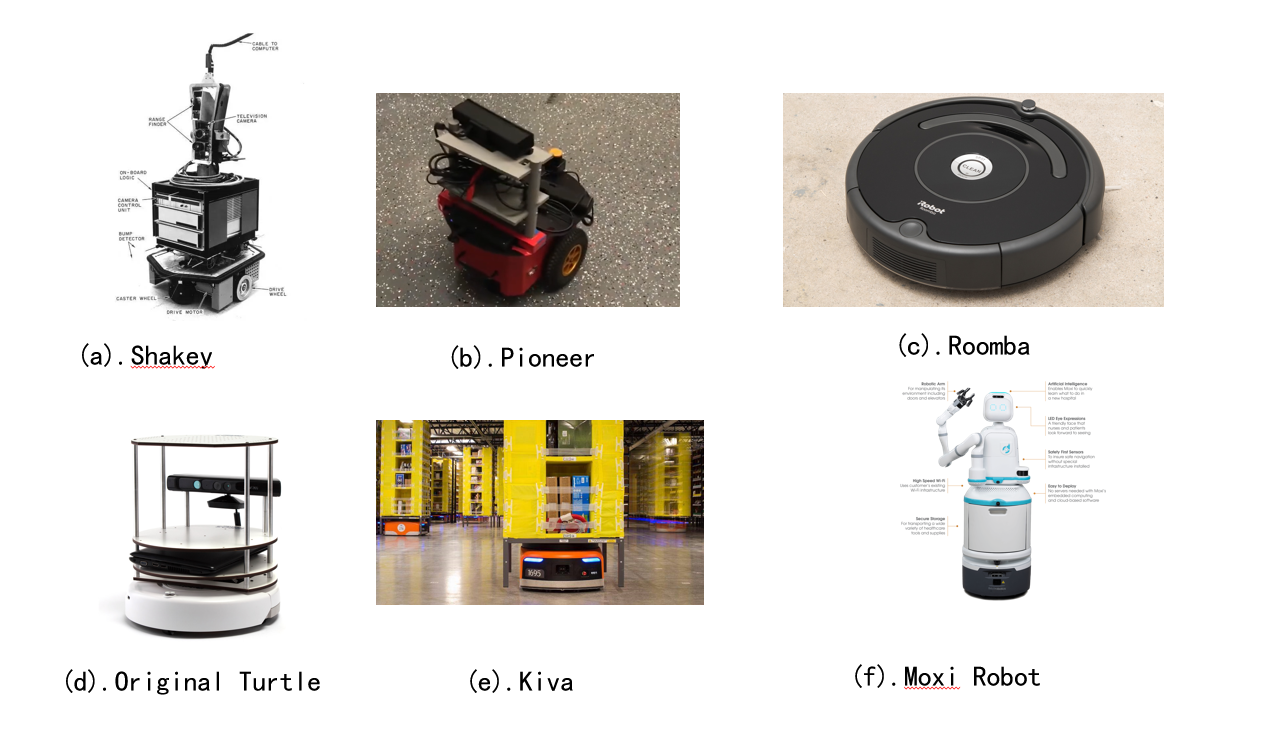
\includegraphics[scale=0.5]{indoorRobot.png}
  \caption{室内移动机器人代表作品}
\end{figure}
2000年之后,随着计算机技术的飞跃,移动机器人迎来了发展的黄金期,仅在10年以前,涌现出的优秀代表作品数不胜数,这个时期也是移动机器人逐渐进入商用的关键时期,iRobot公司于2002年推出一款机器人,名为Roomba\cite{jones2006robots},它可以通过红外线、声音、激光雷达等多种传感器来感知周围环境,实现自主导航和障碍物避免。机器人采用的导航算法是墙隅检测算法(Wall Following Algorithm),它可以通过检测墙面来实现自主运行和避障。由于性能优秀,目前Roomba已经迭代了多代,功能也愈发强大。随后伴随着ROS系统一并问世的Turtlebot\cite{quigley2009ros}给即将到来的机器人时代注入了更大的动力,它采用激光雷达作为感知器件,也可加入深度相机,使用当时并不成熟的SLAM技术进行定位,导航系统已经初具现在移动机器人导航系统的模式,可在室内进行多种任务的执行,同时为机器人学的研究和发展提供了良好的硬件方案。亚马逊旗下的Robotics公司推出了专为物流运输而设计的移动机器人Kiva\cite{weidinger2018storage},它的导航系统基于自主引导技术,采用二维条码标识(2D barcodes)的方式实现自主定位和导航。仓库地面上铺设了一些特殊的标记,每个标记都有独特的标识码。机器人通过底部的摄像头识别这些标记,从而确定自己在地图上的位置,进而计算出最优路径,避开障碍物,到达指定位置。由于其工作环境主要是室内仓库,因此采用这种条码式的标记引导导航十分适合。除了电子标签导航方式之外,最新的Moxi\cite{hurst2020social}机器人采用了多种导航技术,包括激光雷达、摄像头、惯性测量单元(IMU)等,以实现高精度的室内定位和导航。具体来说,Moxi机器人采用激光雷达进行地图构建和建立坐标系,同时结合多个摄像头进行实时环境感知和障碍物检测,IMU则用于进行里程计计算和姿态估计。Moxi还使用了机器学习技术,以学习和识别环境中的人和物体,并根据环境变化实时调整行动路径和速度。

\subsubsection{室外移动机器人——大规模场景}
为室外场景设计移动机器人相比于室内来说,因场景规模较大,难度总体上升一个量级,且室外环境多种多样,园区、矿井、野外等室外环境千变万化,这个过程中也涌现出了一大批优秀的移动机器人设计机构及问世的移动机器人。世界上第一台能够自主导航的车型机器人来自于美国斯坦福大学人工智能实验室的一个早期机器人项目,Stanford Cart\cite{moravec1983stanford}配备有激光雷达、摄像头作为感知传感器,并可以基于当前环境做简单路径规划,躲避动态障碍物。但当时受限于技术的瓶颈,Cart的导航系统并不能对环境进行有效感知,仅仅是可以识别地上的白线进行跟随控制,但这样已经是耗费了计算系统的大量算力。但Cart的问世极大鼓舞了研究者们对移动机器人乃至自动驾驶的探索热情,并奠定了摄像头在移动机器人领域的感知地位。

在室外矿场环境、自然洞穴以及其他复杂环境下,机器人的导航和移动都将变得困难,为攻克这个问题,美国国防高级研究计划局(DARPA)举办了系列比赛——“地下挑战赛”。该赛事目标是开发出能够在地下环境中自主导航、探测、定位、通讯和合作的移动机器人系统,以提高在复杂环境中的人机协作能力。于2007年参赛的GorundHog\cite{nuchter20046d}是一款由卡内基梅隆大学的机器人研究所(Robotics Institute)开发的移动机器人,配备有Sick型号的前后方向的激光雷达以及360°全向的激光雷达,具备激光感知的同时还备有一个摄像头用于视觉感知。其导航方式是基于激光雷达的SLAM方法激光雷达用于建图和障碍物检测,惯性导航系统则用于估计车辆的位置和姿态。其中导航系统所使用的地图则是执行路径规划和障碍物避免的关键数据。同时CMU团队开发的全套自主开源导航系统算法所使用的机器人CMU-EXPLORATION\cite{cao2022autonomous}是一款多场景导航探索机器人,配备有用于导航与测绘的激光雷达 Velodyne Puck、一个 640×360 分辨率的摄像头和一个基于MEMS 的 IMU,以及一只专门用于状态估计的激光雷达,如图所示。低矮
的车身并搭配两轮差速的运动方式,使该平台能够在狭窄、复杂的空间中快速穿梭,实现在校园、楼层等多种场景下的导航与探索任务\cite{zhu2021dsvp,cao2021tare}。
\begin{figure}[ht]
  \centering
  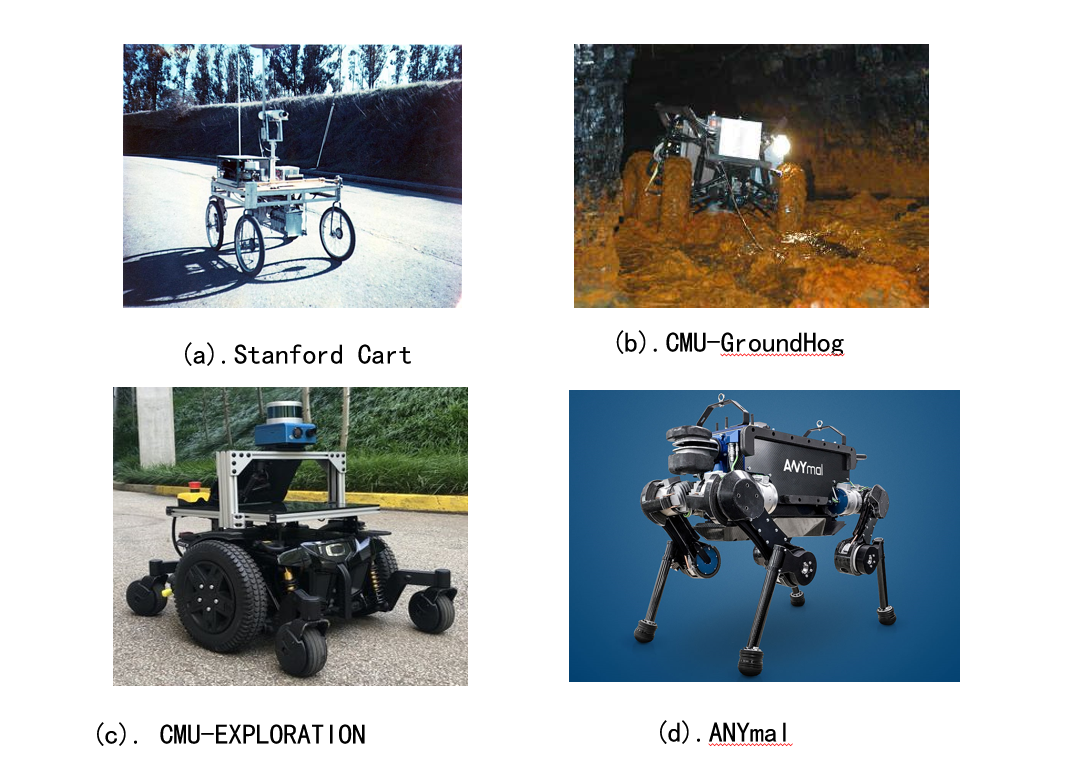
\includegraphics[scale=0.5]{outdoorRobot.png}
  \caption{室外移动机器人代表}
\end{figure}
Boston Dynamics和ANYbotics研发的机器狗已经可在全地形条件下执行任务,由于摆脱了轮子的束缚,使得其在任意条件下的移动都可以实现,通常都配有激光雷达、摄像头、IMU和距离传感器,通过使用深度学习算法和传感器进行导航和避障,两只机器狗的名字分别是Spot和ANYmal\cite{hutter2016anymal}。并且已经有相当多使用Spot和ANYmal进行导航实验的学术成果,例如使用机器狗导航移动和到特定位置抓取物品\cite{zimmermann2021go}。在国内,移动机器人的发展亦如火如荼,例如美团的“大魔袋”移动机器人主要是在小区和园区等封闭室外场景进行区域内的快递、外卖配送。该机器人采用全轮驱动、4轮独立悬挂设计,可以适应各种路况,同时具备强大的动态避障能力。其主要硬件包括雷达、摄像头、激光传感器等,以及可拆卸的货箱。导航系统采用激光雷达和深度相机实现地图构建、定位和路径规划。首先,激光雷达扫描环境获取地形信息,构建地图。然后,深度相机对环境进行实时感知,包括路面状况、障碍物等,用于实现动态避障和路径规划\cite{zhang2022hybrid}。在定位方面,美团大魔袋采用了视觉惯性融合(Visual-Inertial Fusion,VIF)技术,能够实现高精度的自主定位。同时美团大魔袋还具有多种交互方式,如语音、人脸识别等,可以实现人机互动和用户认证等功能。此外,美团大魔袋还支持远程控制和实时监控,保证了配送安全性和效率。

由上述移动机器人的硬件平台研究发展可以看出,移动机器人由室内转向室外并向着多元化使用场景延伸是一个不可阻挡的趋势。计算机技术的大力发展和传感器技术的不断进步是推动移动机器人硬件导航系统不断演进的基础,同时,更加先进的算法适配上更加优秀的硬件系统,使得移动机器人的性能有了质的飞跃,逐渐从实验室模型demo到商业化场景的落地,产生了巨大的实用价值。在硬件系统的进化过程中,导航系统的搭建方式也有了更加科学的规划,主要依靠于激光雷达和摄像头作为感知器件的路线被证明其科学性,辅以IMU等惯性测量技术的卫星定位以及SLAM技术是目前导航系统的主要定位手段,且随着定位技术的成熟化,必将推动导航系统中路径规划和避障技术的持续进步。本文的研究更加关注于当前各大高校、研究机构以及商业公司推出的移动机器人导航系统的架构搭建以及其中涉及到的传感器技术。根据规划,目前阶段使用激光雷达作为在园区场景内导航系统的主要感知传感器是十分科学,因此本文中的系统构建选择Velodyne VLP-16激光雷达作为导航系统的主要感知器件。

\subsection{移动机器人导航避障研究现状}
\subsubsection{静态障碍物避碰}
基于代价地图的方法:这种方法使用代价地图来表示机器人所处的环境,其中每个网格单元格都包含一个代价值,表示该区域对机器人行动的限制程度。代价地图可以通过各种感知设备获得,例如激光雷达、摄像头、超声波传感器等。机器人可以通过在代价地图上进行路径规划来避免碰撞。

基于几何形状的方法:这种方法利用障碍物的几何形状信息,例如大小、形状和位置,来计算机器人的运动轨迹,以避免碰撞。常用的基于几何形状的方法包括多边形轮廓算法和边界表示法等。

基于局部传感器的方法:这种方法利用机器人附近的传感器信息,例如超声波传感器、激光雷达等,检测机器人周围的障碍物。机器人可以通过实时分析传感器数据来规划避障路径,以避免碰撞。

基于网格法的方法:这种方法将环境划分成一个网格,然后根据障碍物的位置将一些网格标记为不可通过,再使用搜索算法进行路径规划。常用的基于网格法的方法包括D算法和A算法等。

\subsubsection{动态障碍物避碰}
导航系统中在园区场景下的动态障碍物碰撞避免方法十分多样,有基于速度障碍(Velocity Obstacle)的方法,基于强化学习的方法,基于模型预测控制(Model Predictive Control)的方法和基于人工势场的方法。

速度障碍的概念被引入移动机器人导航避障领域是2008年时,\citet{van2008reciprocal}提出了一种名为"reciprocal velocity obstacle"(RVO)的方法,用于实现多智能体系统中的实时导航和避障。在移动机器人多智能体避障领域,传统方法是通过预测其他智能体的行动来避免碰撞,但这种方法需要对其他智能体的意图进行预测,而这通常很难。RVO方法不需要对其他智能体的意图运动进行预测,而是通过计算每个智能体之间的速度障碍来避免碰撞。RVO的方法在复杂场景中容易出现局部最优解的问题,于是ORCA\cite{van2011reciprocal}的方案问世,这一方法由RVO的提出团队在原RVO方法的基础上改进得来,称为“Optimal Reciprocal Collision Avoidance”。与RVO不同,ORCA在计算方式上使用线性优化技术来计算最优速度,以便避免碰撞和尽可能地接近目标。同时考虑了其他智能体的速度和位置,通过避免与其他智能体发生碰撞来实现全局最优。ORCA算法的优点在于它能够保证全局最优解,但它的计算复杂度更高。随后,\citet{guy2009clearpath}提出了一种基于GPU加速的多智能体避障算法——ClearPath。该算法使用RVO算法来计算速度,并利用GPU的并行计算能力来加速碰撞检测。实验结果表明,ClearPath算法在性能上比传统的CPU算法要快得多。
\citet{hennes2012multi}提出了一种基于速度障碍范式的多机器人碰撞避免系统。通过在每个智能体上使用自适应蒙特卡罗定位来减轻对每一个障碍物精确感知的要求。因现实的实现不可能做到对周边动态的完美感知,需要进一步扩展来处理不准确的定位和消息传递延迟。此算法限制了由定位引入的误差,并将无碰撞运动的计算与定位不确定性相结合。这篇文章开始从应用层面考虑ORCA的实用性,为推动ORCA在移动机器人导航避障的实地应用做出巨大贡献。
在实际应用方面,\citet{snape2010smooth}提出了一种用于多个独立机器人在差动驱动约束下进行平滑和无碰撞导航的方法。该算法基于最优互惠碰撞避免公式,并保证了机器人轨迹的平滑性和局部无碰撞路径。此方法在运用中结合了差速转轮模型,将ORCA在差速转轮模型约束下进行计算。在其之后,使用此研究结论进行实地实验的结果均证明了算法的有效性。
在此基础之上,\citet{alonso2012reciprocal}提出了一种自行车模型的互相碰撞避免算法(B-ORCA),基于移动机器人的ORCA的概念,但进一步保证了在类似汽车的运动约束下的无碰撞运动。B-ORCA算法的基本原理更广泛地适用于其他运动模型,因为它将速度障碍与通用跟踪控制相结合。通过多个类似汽车的机器人之间的几个仿真实验验证了碰撞避免方面的理论结果。
\citet{snape2014smooth}描述并评估了两种用于多个独立差动驱动机器人的平滑和无碰撞导航的算法。文章基于速度障碍和加速度-速度障碍扩展了互惠碰撞避免算法。并在多个差速机器人上进行了实验,实验证明了文章所提的方法的有效性和实用性。



\subsection{研究现状分析}
目前移动机器人的导航系统的在架构和硬件体系方面已经相当成熟,不同的系统架构可以支持移动机器人在不同的场景下开展导航任务,但对于不同的任务场景之间,移动机器人的导航系统并不能依照同一范式进行支撑或者构建。因此,这给移动机器人在不同场景下的应用以及技术支持带来了巨大的困难。在小规模场景下的工作的移动机器人系统很难通过一定的模块更改适用在大规模的场景之下,大规模场景下的移动机器人导航系统又不像小场景下的移动机器人导航一般只考虑局部规划即可,还需要进行全局范围内的规划。因此我们期望有一种通用的移动机器人导航体系架构,在这个体系架构下,无论是小规模场景的移动机器人导航系统还是应用于园区的导航系统,均可以通过系统的模块更改做相应的算法适配。遗憾的是,目前的开源机器人系统完全依赖于对特定环境的适应,而不将移动机器人的导航系统统一到某个架构下,所以我们的工作虽然是针对于园区场景展开,但是注重了模块之间的独立性和二次开发。经过简单的更改便可以将系统应用于小规模场景。

同时在园区内应用时,关于移动机器人在园区场景下的穿越多动态区域时规划混乱问题,本文发现关于ORCA的讨论一直处于理论和实际应用的边界之中,即使当前的研究已经深入到ORCA和深度学习等人工智能方法结合,但仍然在实际应用中存在巨大间隙,未解决ORCA与阿克曼模型之间存在的约束冲突问题。同时目前的研究在进行ORCA的计算之时,没有实地导航系统的研究佐证,本文期望在导航系统的局部规划中有机嵌入ORCA避障模块,使得园区的移动机器人在进入多动态区域时,以导航系统自带的基于运动元的规划避障方式为主,为ORCA提供当前导航系统下的最优参考速度,基于此最优参考速度,开展ORCA的线性计算,并且反馈得到的计算结果用以与导航框架和阿克曼模型进行二次约束处理,最终得到避障规划结果。同时由于ORCA的计算消耗是巨大的,且目前的研究都是基于已知目前移动机器人周围所有动态物体的前提下进行的,不能有效解决突发情况,例如园区内随时可能出现的突入场景的动态障碍物,因此本文将动态点云的避障同时引入ORCA的方法之中,以导航系统的本身的避障为ORCA算法提供突发动态障碍物的解决方案,并为ORCA算法的最优速度提供参考初值;而ORCA算法则去掉对静态障碍物的计算,负责在阿克曼模型约束之下计算穿越多动态区域的最佳速度。

\textcolor{red}{Give a description of the above}

\section{研究内容}
据上所论,本文的研究主容主要是基于移动机器人的导航系统研究现状——不同场景下设计的移动机器人之间很难互用,移动机器人导航系统目前存在的多种多样的设计方案,且设计方案之间难以协调沟通,同一设计方案中各模块协调性不足等问题,提出一种多层级设计思路的导航方法,此方法由园区移动机器人的导航问题为切入点,将全局性的导航和局部性的导航子系统分模块设计,并且各系统内部模块之间独立工作,可以任意对定位、避障等模块进行二次开发。因为导航系统具备有适应大小规模场景的导航通用架构,易于进行方案的移植。在导航方法的研究与设计过程中,结合了多种性能优越的类别算法,例如底层地形分析与点云聚类算法以及高层中全局地图构建过程的栅格占据状态贝叶斯估计法则与全局路径规划的A*算法。此系统模式简明,性能优越,在园区场景下的测试过程中表现良好。无论是全局的路径规划任务还是小规模的室内规划任务均可出色完成。系统的亮点在于不依靠单一的路径规划算法解决全局状态下的导航问题,使用“多段规划”思想将全局状态下的导航任务以高层和底层两个导航子系统做切分,高层将全局规划任务划分为各个小规模区域内的局部规划任务,再由底层导航以局部规划形式完成小规模区域内的导航。
关于导航系统的研究主要分为两个子导航系统的方法:

1.高层导航方法:以Velodyne VLP-16激光雷达为传感器,采集园区场景下的数据集,并提取数据集中的可行驶区域,并去除其中的动态物体信息,保留全局场景中存在的静态可行驶区域部分,将可行驶区域以点云地图、栅格地图和拓扑地图的形式存储起来,作为离线的先验地图。
高层导航中的路径规划模块读取先验地图,当得到任务目标的终点位置,通过全局定位系统确定自身位置,启动全局场景下的规划,规划在静态的先验地图上进行,且规划只针对于可行驶区域,因此规划出的路径不受实时情况的干扰,只考虑路径的代价。
随后规划模块会根据自身定位与目标点位置规划出一条全局路径$PATH$,保留为一系列路径点,设任意一个路径点为$P_i$,则$P_i$ $\in$ $PATH$,路径点随后会按照车身所处位置,由近及远逐渐下发给底层导航,直至$PATH$中最后一点下发完毕。

2.底层导航方法:底层导航的核心是局部规划器模块,在接收到高层导航下发的路径点之后,立即开始工作。首先底层导航的局部点云构建模块会构建出移动机器人周围一定范围内的点云环境,然后根据局部点位模块,底层导航会掌握此刻移动机器人在环境中的位姿,以及局部环境中$P_i$的位置。移动机器人为通用阿克曼底盘模型,实现离线构建的以后轮中心为base\_link的运动元路径组,所有的运动元满足阿克曼模型约束,根据自身与目标点$P_i$的朝向角度差距,选择其中的某一条路径,选择算法基于朝向角度偏差、障碍物距离等权重后综合分析。选择出路径的情况下,根据构建的运动元选择对应的转向角度与速度,运动控制模块开始工作,通过CAN盒驱动程序将运动速度与转向角度解算为底盘可识别的数字驱动信号,数字驱动信号会驱动电机并控制转向轮,完成行为的表达。循环往复,当$PATH$中最后一个路径点的抵达任务完成之后,整体系统结束运行。

以上便是两个子系统的导航方法与设计思路。此系统已具备在静态环境以及极少动态障碍物的情况进行导航的能力。但当系统运行在园区多动态场景下时,因路底层规导航采用的路径规划模块和避障模块耦合度较高,此时多动态的移动性将会使系统陷入规划混乱和避障提前裕量不足的困境,甚至可能会因此陷入局部最后的死局。

针对园区场景下穿越多动态障碍物区域时出现的避障不鲁棒或者局部规划混乱的问题,基于现有导航框架,提出了一种基于ORCA与运动元规划法相结合的动态导航避障方法。此方法的规划基于底层导航的规划路径与移动方向,将此方向设置为ORCA方法的最优速度方向,动态避障模块根据周围目前的动态障碍物的速度,规划出移动机器人碰撞避免的速度集合,在此速度集合中根据最优速度选择出备用速度。此速度集合由ORCA库的默认圆模型计算而来,需要对速度集合结合阿克曼模型进行二次筛选。若备用速度不满足阿克曼模型约束,则取备用速度的方向和阿克曼模型约束的最大角度进行方向矫正,若备用速度方向正确,若备用速度方向约束满足,则按照模型约束选择运动元中最接近备用速度的一条路径方向,然后辅以ORCA库计算出的速度大小。通过对周围动态物体运动信息的不停感知分析,其园区内动态物体为行人和车辆的前提下,速度方向不会突变且有一定延续性,此动态障碍物碰撞避免模块可以最小路径代价规划出穿越多动态障碍物区域的局部路径。此局部路径同时满足了阿克曼模型约束下的角度约束与ORCA算法下的最小代价,可以使底层规划模块顺利穿越多动态障碍物区域到达目标点$P_i$。


\section{论文组织结构}
论文的组织架构以建立一种通用的导航系统方法框架为指导思想,不按照功能模块,例如定位、建图或者路径规划等来划分,而按照功能层级划分为底层和高层两部分。第三章详细介绍了高低层导航方法中所涉及到的各种算法细节以及方法等,第四章针对第三章中导航方法存在的无法穿越多动态区域的问题,创新提出一种多动态障碍物的导航避障方法,此避障方法作为功能模块仅在检测到多动态障碍物时启动,离开多动态障碍物区域后则停止运行,因此既是方法又是单独的创新设计,故单列为一章。第五章内容是在前面两章方法设计的基础之上,搭建移动机器人的硬件系统,并将此系统之间的信息传递分别以硬件系统的数据流向和软件系统的消息流向方式进行展现,并且附上相应的实地实验。

论文的架构图可如下表示:

\subsection{章节结构图}
\begin{figure}[ht]
  \centering
  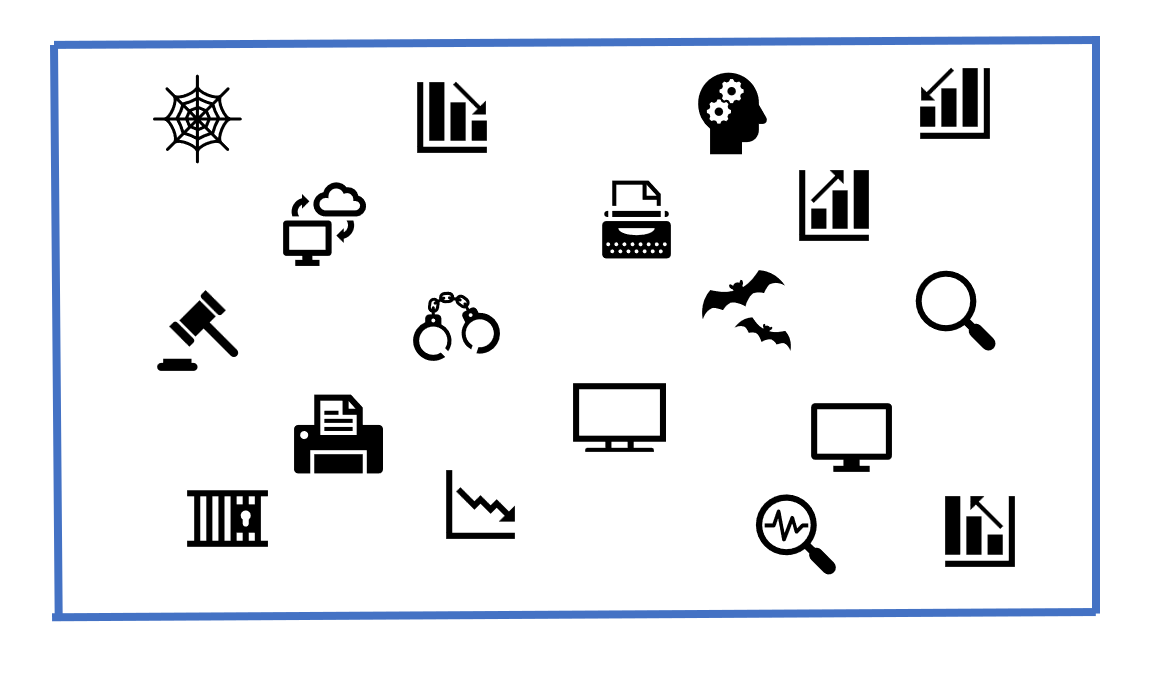
\includegraphics[scale=0.5]{template.jpg}
  \caption{模板图片}
\end{figure}




\section{脚注}

\subsection{二级节标题}

\subsubsection{三级节标题}

\paragraph{四级节标题}

\subparagraph{五级节标题}

Lorem ipsum dolor sit amet, consectetur adipiscing elit, sed do eiusmod tempor
incididunt ut labore et dolore magna aliqua.
\footnote{Ut enim ad minim veniam, quis nostrud exercitation ullamco laboris
  nisi ut aliquip ex ea commodo consequat.
  Duis aute irure dolor in reprehenderit in voluptate velit esse cillum dolore
  eu fugiat nulla pariatur.}